%  !TeX  root  =  user_guide.tex 

\section{Extension d'Analyse Raster de Terrain}

% when the revision of a section has been finalized, 
% comment out the following line:
%\updatedisclaimer

%The Raster Terrain Modelling plugin can be used to calculate the slope, aspect, ruggedness, and
%total curvature for digital elevation models (DEM). It is very simple to handle and provides an
%intiuitive graphical user interface for creating new raster layers (See Figure
%\ref{fig:raster_terrain_dialog}).
L'extension d'analyse de terrain basée sur les rasters peut être utilisée pour calculer la pente, l'aspect, la rugosité et la courbure totale d'un modèle numérique d'élévation (DEM). Sa facilité d'utilisation et son interface graphique intuitive permettent de créer de nouvelles couches raster (voir figure \ref{fig:raster_terrain_dialog}).

%The plugin requires the following parameters to be specified before running:
L'extension requiert les paramètres suivants pour pouvoir être utilisée :

%\begin{itemize}
%\item[Analysis :] Can be one of slope, aspect, ruggedness, or total curvature
%\item[Input layer :] Specify the input raster from a list of loaded
%raster layers.
%\item[Output layer :] Specify a name and path for the output raster file.
%\item[Output format :] Specify a format type for the output raster file (Default is GeoTiff).
%\end{itemize}
\begin{description}
\item[Analyse :] Cela peut être une analyse de la pente, l'aspect, la rugosité ou de la courbure totale
\item[Couche en entrée :] Specifiez la couche raster à charger depuis une liste
\item[Couche en sortie :] Specifiez un nom et un chemin pour le raster qui sera produit
\item[Format en sortie :] Specifiez un format pour ce raster (celui par défaut est le GeoTiff)
\end{description}

%Slope: Calculates slope angle for each cell in degrees (based on first order derivative estimation).
Pente : Calcule l'angle de la pente pour chaque cellule (en degrés, en se basant sur une estimation dérivée de 1er ordre).
%Aspect: Exposition (starting with 0 for north direction, in degrees counterclockwise).
Aspect : Calcule l'exposition (en degrés dans le sens horaire inverse et en commençant par 0 pour une direction nord).
%Ruggedness factor: A quantitative measurement of terrain heterogeneity.
Facteur de rugosité : Une mesure quantitative de l'hétérogénéité du terrain.
%Total curvature: A curvature measure that combines plan- and profile curvature.
Courbure totale : Une mesure de la courbure qui combine les courbes de plan et de profil.

%\begin{figure}[ht]
%   \begin{center}
%   \caption{Raster Terrain Modelling Plugin \nixcaption}\label{fig:raster_terrain_dialog}\smallskip
%   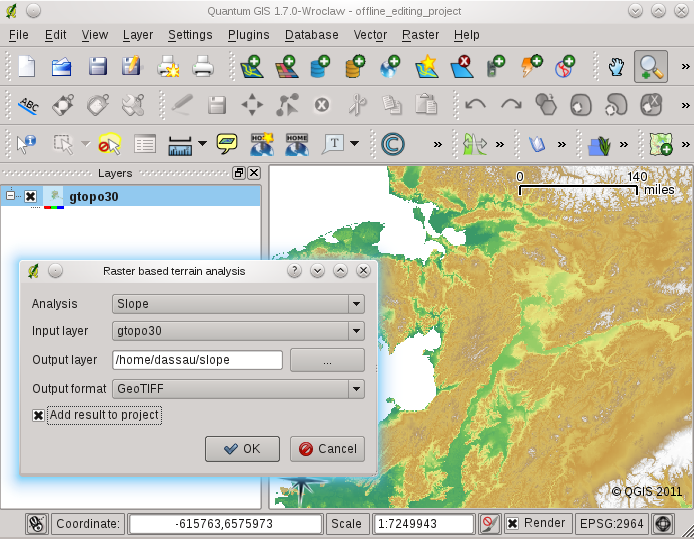
\includegraphics[clip=true, width=9cm]{raster_terrain_dialog}
%\end{center}  
%\end{figure}
\begin{figure}[htb]
\centering
   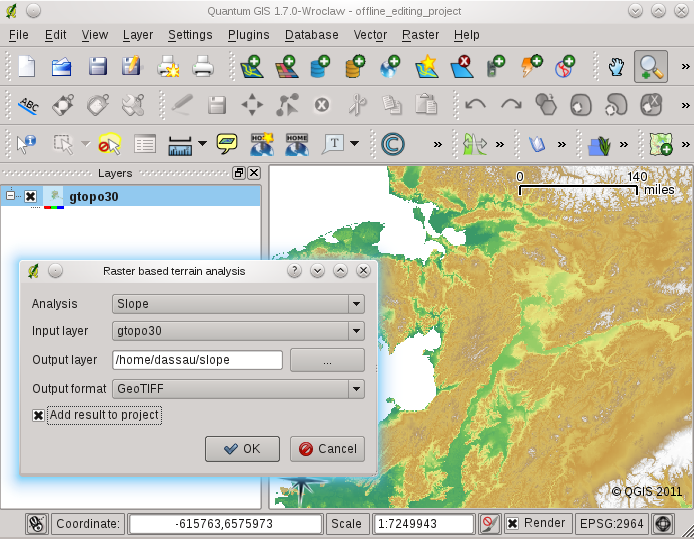
\includegraphics[clip=true, width=6cm]{raster_terrain_dialog}
   \caption{Extension d'Analyse Raster de Terrain \nixcaption}\label{fig:raster_terrain_dialog}
\end{figure}

%\minisec{Using the plugin}\label{raster_terrain_usage}
\minisec{Utiliser l'extension}\label{raster_terrain_usage}

%\begin{enumerate}
%  \item Start \qg and load a DEM raster layer. 
%  \item Load the Raster Terrain Modelling plugin in the Plugin Manager (see Section 
%  \ref{sec:load_core_plugin}) and click on the \toolbtntwo{raster_terrain}{Raster Terrain
%Modelling} icon which appears in the \qg toolbar menu. The Raster Terrain Modelling plugin dialog
%appears as shown in Figure \ref{fig:raster_terrain_dialog}.
%  \item Select an analysis method (e.g. \dropmenuopt{Slope}).
%  \item Specify an output file
%path, and an output file type.
%  \item Click \button{Ok}.
%\end{enumerate}
\begin{enumerate}
  \item Lancez \qg et chargez une couche raster DEM.
  \item Chargez l'extension via le gestionnaire d'extension (voir section \ref{sec:load_core_plugin}) et cliquez sur l'icône \toolbtntwo{raster_terrain}{Analyse de terrain} qui apparaît dans la barre d'outils. La fenêtre de l'extension s'affiche telle que montrée dans la figure \ref{fig:raster_terrain_dialog}.
  \item Sélectionnez une méthode d'analyse (p. ex. \dropmenuopt{Pente}).
  \item Spécifiez un chemin de sortie et le type de fichier produit.
  \item Cliquez sur \button{Ok}.
\end{enumerate}